\documentclass[a4paper, 11pt]{article}
\usepackage{comment} 
\usepackage{fullpage}
\usepackage{amsmath} 
\usepackage{amssymb} 
\usepackage{mathtools}
\usepackage{siunitx}
\usepackage{xfrac}
\usepackage{icomma}
\usepackage[section,below]{placeins}
\usepackage[labelfont=bf,font=small,width=0.9\textwidth]{caption}
\usepackage{subcaption}
\usepackage{graphicx}
\usepackage{grffile}
\usepackage{float}
\floatplacement{figure}{htbp}
\floatplacement{table}{htbp}
\usepackage{booktabs}
\usepackage{hyperref}
\usepackage{pdfpages}
\sisetup{separate-uncertainty=true}

\begin{document}
\noindent
\centerline{\small{\textsc{Michigan State University}}} \\
\large{\textbf{CMSE 823 – Numerical Linear Algebra \hfill Spring 2020 \\
Final Programming Project Write-Up} \\
Alexander Harnisch \\
\noindent\makebox[\linewidth]{\rule{\textwidth}{0.4pt}}

Please find the solutions to Questions 1 and 2 as well as the explanation of my
idea for Question 6 in handwritten form in \textit{handwritten\_part.pdf}.

A general comment: For all implementations I used the efficient
\textsc{NumPy} implementations for solving linear systems and for computing the
QR factorization as part of the algorithms. I might as well have used my
implementations from the homework. However, those are significantly slower.

\section*{Question 3}
Our matrix is positive definite and
symmetric, therefore to find the smallest eigenvalue using inverse iteration,
we do not need to shift it. To numerically demonstrate the second order
convergence of the smallest eigenvalue to the true smallest eigenvalue
$\lambda_\textup{min} = \frac{p}{4} + q$ (here and for the other questions), I
plot 
\begin{equation}
  \frac{\vert \lambda_\textup{min}^h - \lambda_\textup{min}\vert}{h}
\end{equation}
against $h$, which should show a linear relation if the convergence is
indeed quadratic. Figure~\ref{fig:3} clearly shows this behaviour and therefore
demonstrates the second order convergence.
\begin{figure}
  \centering
  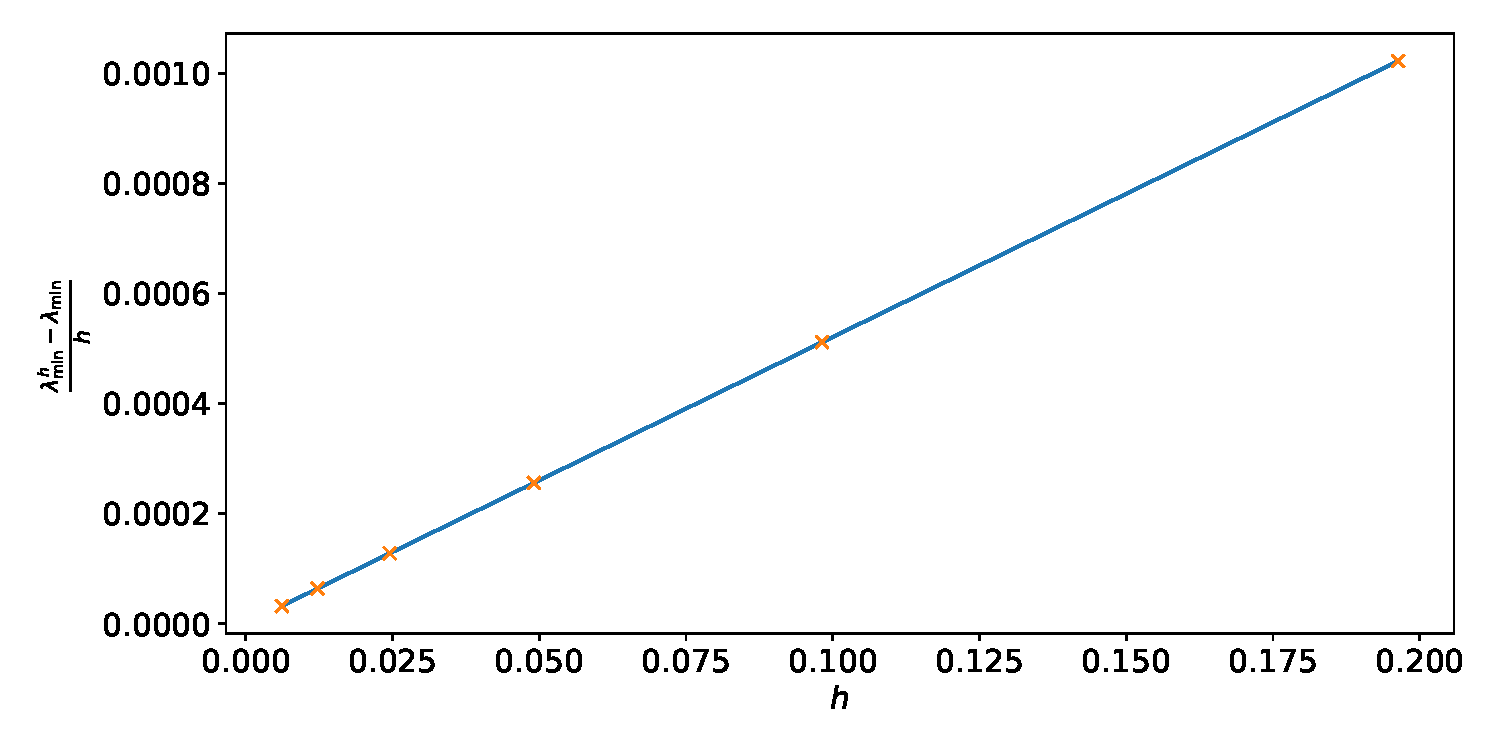
\includegraphics[width=\textwidth]{../code/3.pdf}
  \caption{Error of the smallest eigenvalue over $h$ in dependence of $h$ for
  $p = 1$ and $q = 5$.}
  \label{fig:3}
\end{figure}

\FloatBarrier
\section*{Question 4}
To find the smallest eigenvalue using the shifted power method, we ideally want
to choose the shift to be as close as possible to the eigenvalue with largest
absolute distance to the smallest eigenvalue. Again, since the matrix is
symmetric and positive definite, it only has positive eigenvalues and therefore
the best choice is its largest eigenvalue. So I found it is actually best and
fastest just to compute that one first and then use it as a shift. The result
in Figure~\ref{fig:4} again demonstrates the second order convergence of
$\lambda^h$, as expected.
\begin{figure}
  \centering
  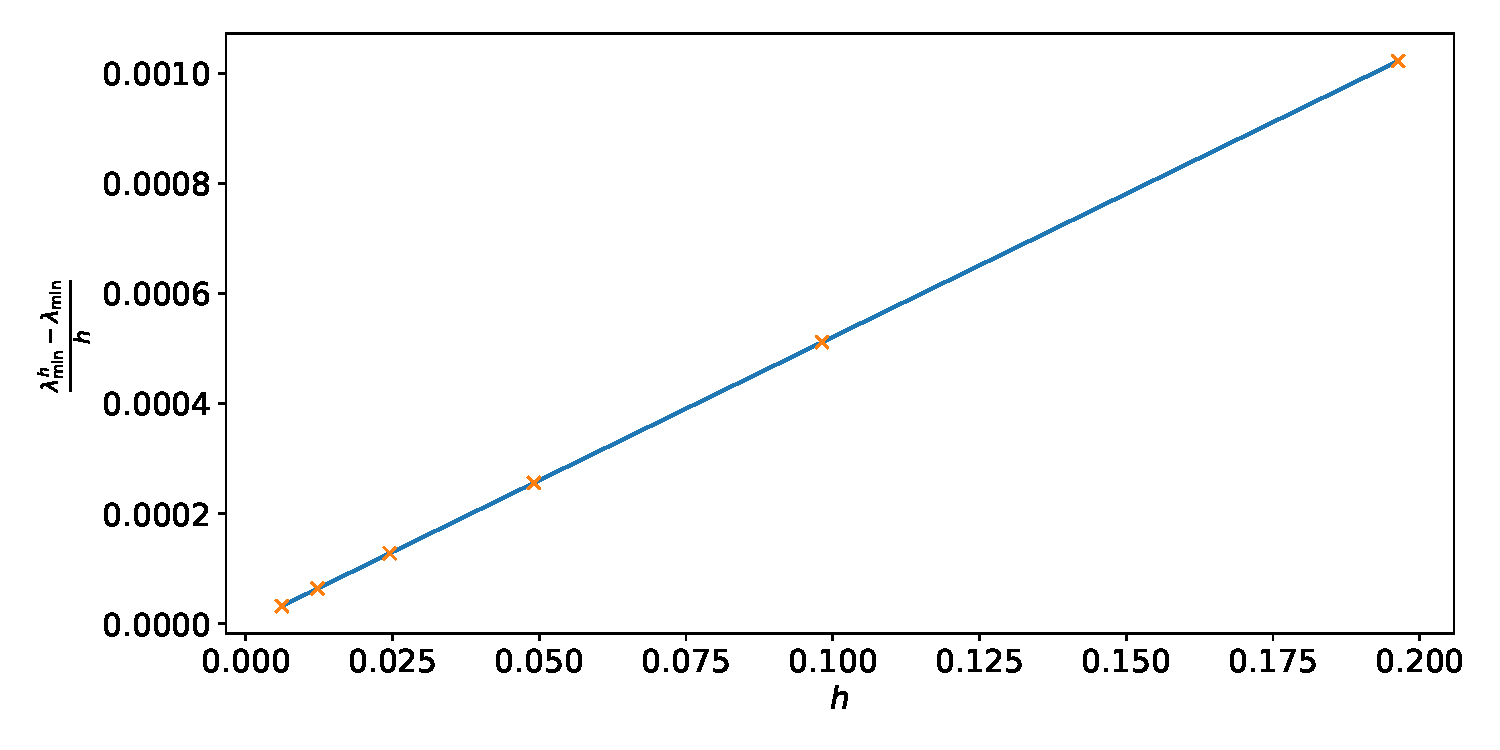
\includegraphics[width=\textwidth]{../code/5.pdf}
  \caption{Error of the smallest eigenvalue over $h$ in dependence of $h$ for
  $p = 1$ and $q = 5$.}
  \label{fig:4}
\end{figure}

\FloatBarrier
\section*{Question 5}
I based the QR iteration with deflation algorithm on Algorithm 28.2 from the
textbook. Just without shifts, as the Rayleigh shift does not seem to work in
this case, because it does generally not converge for symmetric matrices (I
implemented it and it did not converge for large $N$). So I implemented two
versions: A recursive and an iterative one. The recursive one checks in every
iteration if \textbf{any} of the sub-diagonal elements are sufficiently close
to zero, and if so continues recursively with the two uncoupled sub-matrices as
suggested in the slides. However, it turns out for this matrix the element
first being eliminated is always the one in the last row anyway, even without
using the Rayleigh coefficient as a shift. The iterative implementation makes
use of that and is significantly faster. Both return the same result shown in
Figure~\ref{fig:5}, again demonstrating the expected convergence.
\begin{figure}
  \centering
  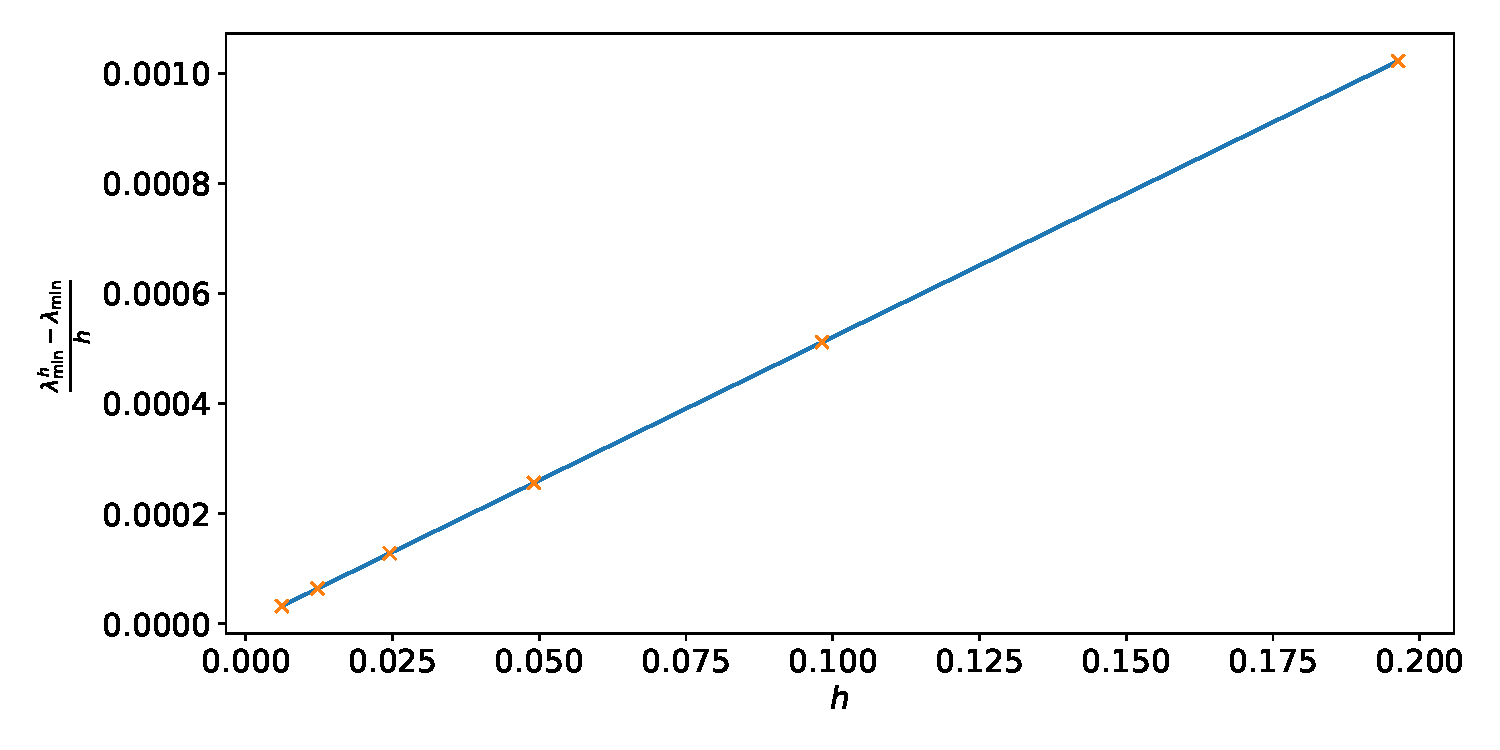
\includegraphics[width=\textwidth]{../code/5.pdf}
  \caption{Error of the smallest eigenvalue over $h$ in dependence of $h$ for
  $p = 1$ and $q = 5$.}
  \label{fig:5}
\end{figure}

\FloatBarrier
\section*{Question 6}
My idea for the method to solve the generalized eigenvalue problem is explained
in the handwritten part. Essentially it is a modified version of the inverse
iteration, with the only addition of applying matrix $B$ to the intermediate
vectors.  The result in Figure~\ref{fig:6} once again confirms the quadratic
convergence.
\begin{figure}
  \centering
  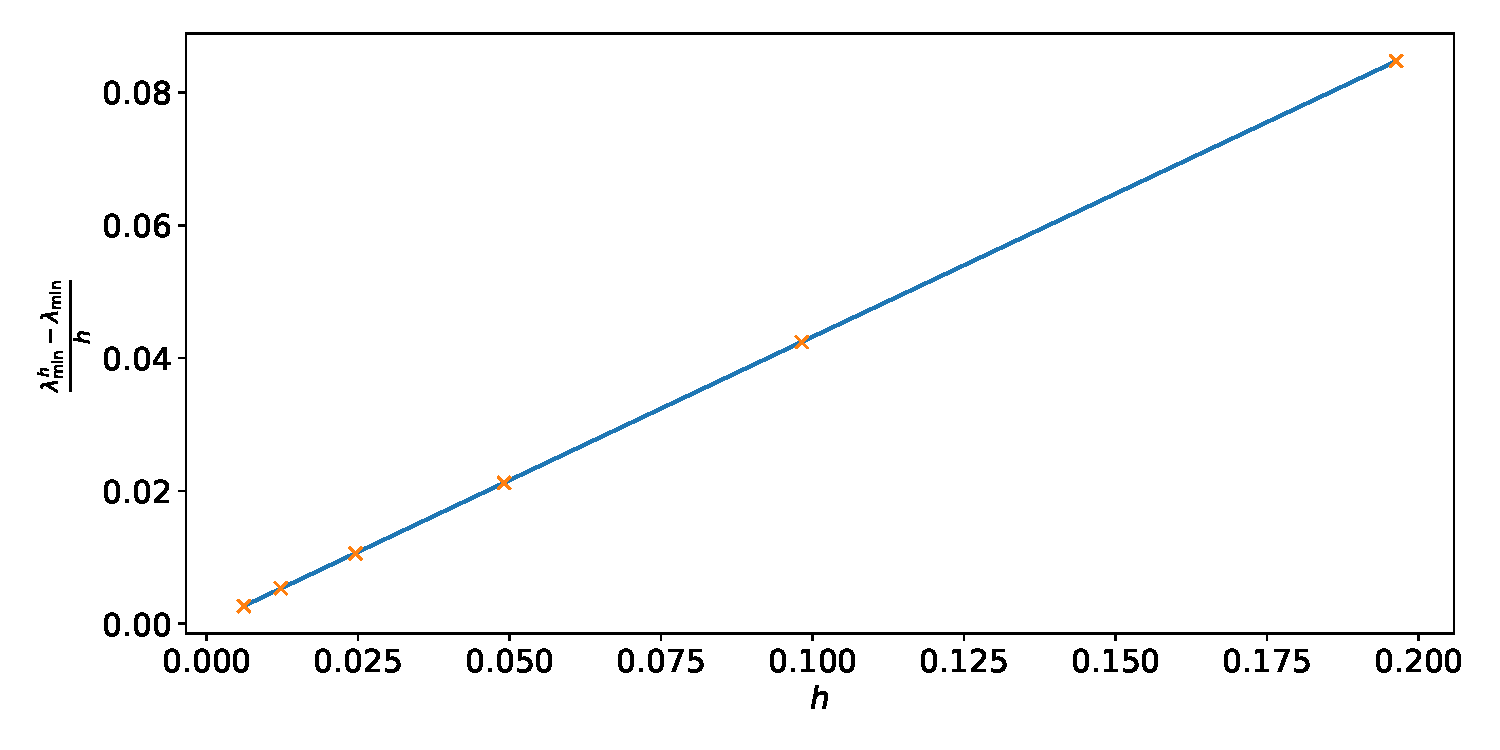
\includegraphics[width=\textwidth]{../code/6.pdf}
  \caption{Error of the smallest eigenvalue over $h$ in dependence of $h$ for
  $p = 1$ and $q = 5$.}
  \label{fig:6}
\end{figure}
\end{document}
